% Changing book to article will make the footers match on each page,
% rather than alternate every other.
%
% Note that the article class does not have chapters.
\documentclass[10pt,twoside,twocolumn,openany]{book}
\usepackage[bg-full]{dnd} % Options: bg-a4, bg-letter, bg-full, bg-print, bg-none.
\usepackage[english]{babel}
\usepackage[utf8]{inputenc}
\usepackage{calc}
\usepackage{tikz}
\usepackage{graphicx}
\usetikzlibrary{calc}
\usepackage{wrapfig}
\usepackage{subfiles}

\graphicspath{{images/}}

% Start document
\begin{document}
\fontfamily{ppl}\selectfont % Set text font

% Your content goes here

% Comment this out if you’re using the article class.
\chapter{Character: ???}

\begin{tikzpicture}[remember picture,overlay]
  \node[anchor=south west,inner sep=0pt] at ($(current page.south west)$) {
     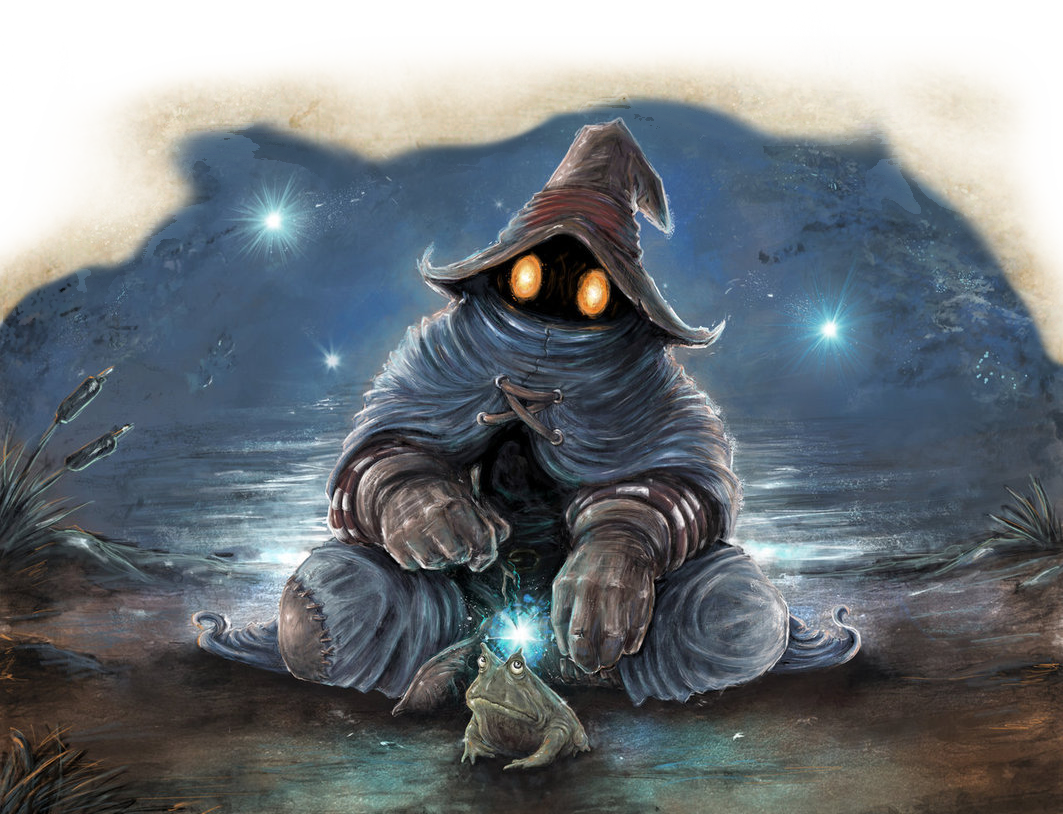
\includegraphics[width=\paperwidth]{black-mage-transparent}
  };
\end{tikzpicture}

{\vspace{-3em}}

\section{Main Section}
\lipsum[1] % filler text

\newpage

\lipsum[1] % filler text

\subsection{Fun with boxes}

\begin{quotebox}
	As you approach this template you get a sense that the blood and tears of many generations went into its making. A warm feeling welcomes you as you type your first words.
\end{quotebox}

\newpage

\begin{commentbox}{Neat Green Box!}
	\lipsum[1]
\end{commentbox}

\subtitlesection{Weapon, +1, +2, or +3}
{Weapon (any), uncommon (+1), rare (+2), or very rare (+3)}

\newpage % Acts as columbreak because of twocolumn option; for pagebreak use \clearpage

% For more columns, you can say \begin{dndtable}[your options here}.
% For instance, if you wanted three columns, you could say
% \begin{dndtable}{XXX}. The usual host of tabular parameters are
% aailable as well.
\header{Nice table}
\begin{dndtable}
	   \textbf{Table head}  & \textbf{Table head} \\
	   Some value  & Some value \\
	   Some value  & Some value \\
	   Some value  & Some value
\end{dndtable}

\begin{paperbox}{Do the Players need direction?}
	\lipsum[1]
\end{paperbox}

% You can optionally not include the background by saying
% begin{monsterboxnobg}
\begin{monsterbox}{???}
	\textit{Small lightfoot halfling (doppleganger), lawful evil}\\
	\hline
	\basics[%
	armorclass = 13,
	hitpoints  = 13,
	speed      = 20 ft
	]
	\hline
	\stats[
	STR = \stat{12}, % This stat command will autocomplete the modifier for you
	DEX = \stat{14},
	CON = \stat{10},
	INT = \stat{13},
	WIS = \stat{12},
	CHA = \stat{20}
	]
	\hline
	\details[%
	% If you want to use commas in these sections, enclose the
	% description in braces.
	% I’m so sorry.
	senses = {Darkvision 60 ft},
	languages = {Common, Erlang},
	conditionimmunities = {Charmed},
	]
	\hline \\[1mm]
	\begin{monsteraction}[Monster-super-powers]
		This Monster has some serious superpowers!
	\end{monsteraction}
	\monstersection{Actions}
	\begin{monsteraction}[Generate text]
		This one can generate tremendous amounts of text! Though only when it wants to.
	\end{monsteraction}

	\begin{monsteraction}[More actions]
	See, here he goes again! Yet more text.
	\end{monsteraction}
\end{monsterbox}

\clearpage

% Comment this out if you’re using the article class.
\chapter{Appendix}

\subfile{sections/doppelganger}

\section{Warlock}
\subfile{sections/warlock}

% End document
\end{document}
